

\chapter{System description}

This section discusses the implementation of the project with
references to the source tree. See figure \ref{fig:overview}.
Note that the source tree has been refactored by E.W. Thomassen
to better fit with other PyPy projects. This section discusses how
and where the specific functionality is implemented. Note that there
are a number of problems with the current implementation, and that
these are discussed in chapter \ref{chap:conc}

The toplevel of the source tree contains a README file and a folder
called "pyhaskell".

\section{Pyhaskell toplevel}

The toplevel of the source tree contains 3 main programs. "main.py",
"makegraph.py" and "runtests.py".

"main.py" is the entrypoint of the compilation system. It defines
the target for the RPython translation tool, imports the \emph{builtin}
functionality and the main function begins the interpretation of the
JSCore program.

The program "makegraph.py" contains a JSON parser and dumps the resulting
JSON tokens to a dot file in order to generate a graph using graphviz.

The "runtests.py" program contains a program that executes all the programs
in the "test/" subfolder and the prints the result of the tests.




\begin{sidewaysfigure}
\begin{figure}[H]
\centering
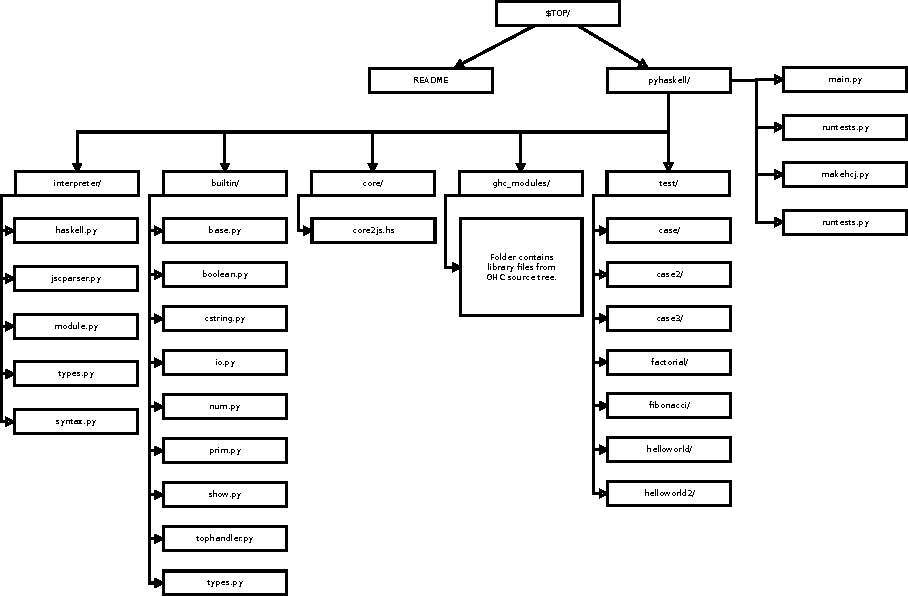
\includegraphics[width=\textheight]{../diags/overview.pdf}

\caption{Overview of source tree}
\label{fig:overview}

\end{figure}
\end{sidewaysfigure}




\section{Interpreter}

The subfolder "interpreter" in "pyhaskell" contains the actuall 
interpreter code, the parser and the module system implementation.

\subsection{haskell}

The file "haskell.py" in the folder "interpreter" contains the
Haskell-Python interpreter, the base of the compilation system.
This section describes the keys of the Haskell-Python implementation.
See figure \ref{fig:coreinterp} for a class diagram.

Haskell-Python consists of a few base classes; 

\begin{itemize}

\item \emph{Symbol} contains a static dictionary of all Symbols. This is 
simply used to compare "names" by their object identity.

\item \emph{HaskellObject} is a base class for all objects handled by the
interpreter.

\item \emph{Value} is a base class for evaluated values.

\item \emph{Constructor} inherits from \emph{Value} and implements an abstract 
base class for constructors with different number of arguments.

\item \emph{ConstructorN} inherits from \emph{Constructor} and is used as the 
base for a number of other Constructor classes created by a function called 
\emph{make\_arg\_subclass}. This function is again called by another function
called \emph{make\_constructor} that creates a Constructor based on the length
of the list it receives as argument. And this function (\emph{make\_constructor})
is called by another function \emph{constr} takes the name-argument (a string)
and looks it up in the list of symbols to create the actual Constructor. So the
actual Constructor is created by a coll to the function \emph{constr(name, *args)}.

\item \emph{AbstractFunction} inherits from \emph{Value} and is the base class for 
the functions of Haskell-Python. 

\item \emph{Function} inherits from AbstractFunction and defines a user-defined 
Haskell-Python function, it contains a name and a list of \emph{Rules}

\item \emph{Rule} is a field of the Function. It consists of a list of patterns and
an expression. If the function is applied and its arguments matches a pattern, the
expression is evaluated.

\item \emph{Substitution} inhertis from HaskellObject and is the body of a function 
with its numbered variables substitutet by values.

\item \emph{PrimFunction} inherits from \emph{AbstractFunction} and describes a function
implemented at the machine level. A function called \emph{expose\_primitive} is
can be used as a python-decorator to create \emph{PrimFunction} objects.

\item \emph{Var} inherits from \emph{HaskellObject} and describes a Haskell variable. 

\item \emph{NumberedVar} inherits from \emph{HaskellObject}. A \emph{Var} is replaced
by a \emph{NumberedVar} by a call object-function \emph{enumerate\_head} inherited from
\emph{HaskellObject} when creating a \emph{Rule}.

\item \emph{Application} inherits from \emph{HaskellObject} and describes an
abstract base class for Haskell-Python function application. Like the constructor,
classes are created by a function for various number of arguments.

\item \emph{ApplicationN} inherits from \emph{Application} and is used by the function
\emph{make\_application} to create Application classes with various number of arguments.
This function, like \emph{make\_constructor} is used by the function 
\emph{make\_arg\_subclasses} to create Applications with various number of arguments.

\item \emph{Thunk} inherits from \emph{HaskellObject} and represents an unevaluated
function application. 

\item \emph{StackElement} is a base class for the elements of the evaluation stack.

\item \emph{CopyStackElement} inherits from \emph{StackElement} and contains a
\emph{Application}.

\item \emph{UpdateStackElement} inherits from \emph{StackElement} and contains a
\emph{Thunk}. The \emph{Thunk} contained in the object is updated after its 
content has been evaluated.
\end{itemize}

In addition to these classes, the most important functions are;

\begin{itemize}

\item \emph{expose\_primitive} and the following two functions have allready been 
mentioned. \emph{expose\_primitive} can be used as a python-decorator.

\item \emph{constr} creates a \emph{Constructor} object by looking up the "name" in
the dictionary of the \emph{Symbol} class, and selecting the correct sub-class from the
sub-classes generated for \emph{Constructor}.

\item \emph{make\_application} is similar to \emph{make\_constructor}, there is no
need for a wrapper function as it does not have to look up a \emph{Symbol}.

\item \emph{main\_loop} is the main function, it reduces a Haskell-Python 
\emph{Application} to a \emph{Value}. The function \emph{evaluate\_hnf} is
simply a wrapper for the \emph{main\_loop function}
\emph{main\_loop}.

\end{itemize}


\begin{sidewaysfigure}
\begin{figure}[H]
\centering
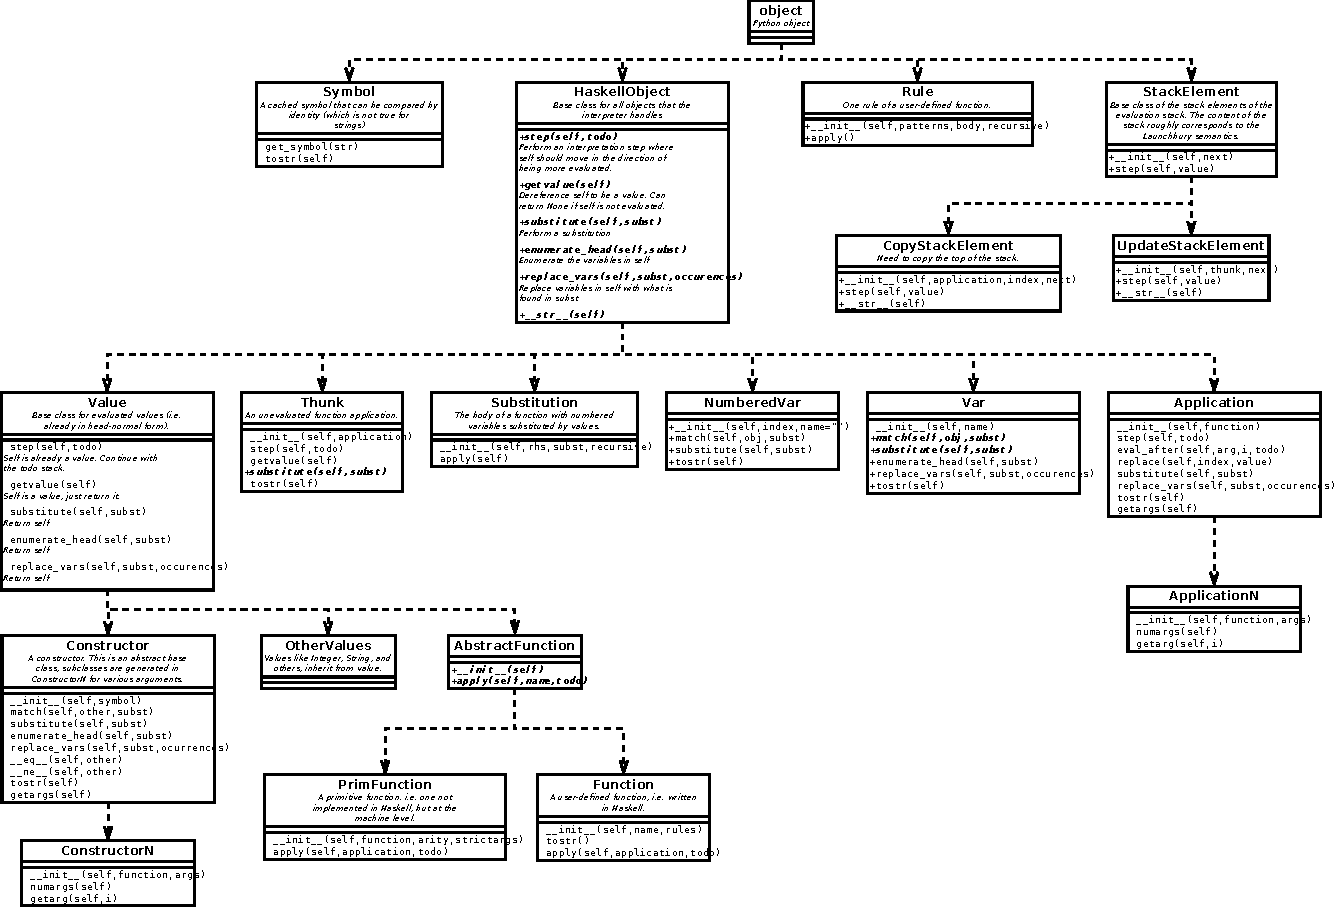
\includegraphics[width=\textheight]{../diags/core-interp.pdf}

\caption{Haskell-Python class diagram}
\label{fig:coreinterp}

\end{figure}
\end{sidewaysfigure}



\subsection{primtypes}

The file "primtypes.py" in the folder "interpreter" contains the primitive types
for the Haskell-Python interpreter. The types implemented inherit from the
\emph{Value} class in "haskell.py".

The following primitive types are implemented;

\begin{itemize}
\item \emph{Char} represents a single Haskell character-value.
\item \emph{Int} represents a Haskell Int value.
\item \emph{Addr} is a memory address. Among other it is used to represent
the String type.

\item \emph{Double} is simply a double precision floating point value.
\item \emph{Float} is simply a single precision floating point value
\end{itemize}

Since these classes all inherit from the Value type of Haskell-Python, 
they have a common interface; they all contain a variable called value that
contain its actual contents. This is currently implemented as a python
variable, so it is not represented like its Haskell equivalent at the low-level.
See listing \ref{lst:int1} for an example of how a primitive value is implemented.

\begin{figure}[H]
\lstset{ %
language=Python,
caption=Python class implementing the Haskell Int Value.,
label=lst:int1
}
\begin{lstlisting}
class Int(haskell.Value):
    _immutable_fields_ = ["value"]

    def __init__(self, integer):
        assert isinstance(integer, int)
        self.value = integer

    def match(self, other, subst):
        value = other.getvalue()
        if value:
            assert isinstance(value, Int)
            if self.value == value.value:
                return haskell.DEFINITE_MATCH
            return haskell.NO_MATCH
        return haskell.NEEDS_HNF

    def __eq__(self, other):
        return (isinstance(other, Int) and self.value == other.value)

    def __ne__(self, other):
        return not (self == other)

    def tostr(self):
        return str(self.value)
\end{lstlisting}
\end{figure}


\subsection{module}

The file "module.py" in the folder "interpreter" contains the basics of the
module system. It contains a single class; \emph{CoreMod}. This class corresponds
to a Haskell Module. A \emph{CoreMod} object contains a name, and three dictionaries.
These dictionaries are called \emph{qvars}, \emph{qtycons} and \emph{qdcons} and they
contain \emph{qualified variables}, \emph{qualified type constructors} and 
\emph{qualified dataconstructors} respectively. When a \emph{CoreMod} object is created
it is at once added to the list of Haskell Modules.

\subsection{jscparser}

The file "jscparser.py" in the "interpreter" folder contains the parser code. 
This code is responsible for loading JSCore files, and creating the AST based 
on the interpreter and module-system implementations.

The parser implementation takes advantage of some of the parsing tools 
available from
the PyPy codebase. By creating a EBNF grammar for JSON, and giving it to a 
function called \emph{parse\_ebnf}, a JSON parser is created.

The resulting parser is a base class called \emph{RPythonVisitor}. The 
RPythonVisitor
class implements \emph{visit} functions for the constructs created by the 
EBNF grammar. For JSON this becomes \emph{visit\_object}, 
\emph{visit\_number} etc.

The result of this is that we have a set of functions that get called when 
visiting JSON constructs. Since JSCore is a description of External-Core 
compatible with JSON this lets us parse the Core programs by branching 
on the visitor functions.


\section{Builtin}

The "builtin/" folder contains all the Haskell library functionality that
have been implemented in Python. Most of this functionality should have been
stored in the subfolder "ghc\_modules" as JSCore files. However, due to some 
issues that are discussed in conclusions and future work, this is not currently
the case.

As an example, the file "num.py" contains the implementation for the generic
Num class. Listing \ref{lst:zmnum} contains the implementation for the
generic minus function. Currently it only supports the Int type. Note that
it takes three arguments, the first argument is used to resolve which 
function actually implements the minus function, and the other two are the
arguments for this function.

\begin{figure}[H]
\lstset{ %
language=Python,
caption=Python class implementing the Haskell Int Value.,
label=lst:zmnum
}
\begin{lstlisting}
@haskell.expose_primitive(3)
def zm( args ):
    ty = args[0]
    a = args[1]
    b = args[2]

    if ty == mod.qvars["$fNumInt"]:
        return haskell.make_partial_app(izhconstr,
            [haskell.make_partial_app(prim.zmzh, [a.getarg(0), b.getarg(0)])])
    else:
        raise NotImplementedError

mod.qvars["-"] = zm
\end{lstlisting}
\end{figure}



\section{Core}

The "core/" folder contains the Haskell program responsible of generating the
JSCore intermediate format. This program is called "core2js". Currently, the
program uses the External-Core parser from the "extcore" Haskell package and
the JSON package to read the Haskell file in External-Core format and dump it
in JSCore format.

\section{GHC modules}

The folder "ghc\_modules" contain the GHC boot libraries. And a script that 
takes all these Haskell modules and uses GHC to create External-Core files
using the "-fext-core" flag and "core2js" to create JSCore files from the 
resulting External-Core files.

The GHC library files are organized exactly as in the GHC source tree. Each
folder in the "libraries/" directory corresponds to a Haskell package. These
packages contain the Haskell modules. E.g. the module "GHC.Tuple" is located
in "ghc-prim/GHC/Tuple.hs".

\section{Tests}

The "test/" directory contains one subdirectory for each test. The
subdirectories contain a single Haskell file with the same name as the
subdirectory (other files are created and put in the directory when running
the test). E.g. the test "fibonacci" is located in the following path:
"test/fibonacci/fibonacci.hs" and after running the test the "fibonacci/"
folder should contain the additional files; "factorial.hcr", "factorial.hi",
"factorial.o" and "factorial.hcj". ".hcj" is the extension used for JSCore
files.


\begin{comment}

\section{Pipeline}
\label{chap:pipe}

This section contains a description of the pipeline currently implemented.

\subsection{Haskell to extcore}

When running a Haskell file using this system, the file is first processed
by GHC.

\subsection{Extcore to JSCore}

\begin{itemize}
\item extcore
\item linkcore ?
\end{itemize}

\subsection{JSCore to Core'}

\subsection{Parsing and interpretation}





\section{Testing}
\label{chap:test}

\subsection{Current testing of interpreter}

The current testing used on the project is done by a python-script that performs
the following actions:

\begin{itemize}

\item For all folders in folder 'test':

\begin{itemize}

\item Compile haskell program with GHC and dumping to external-core

\item Run the core2js program on resulting external-core file

\item Run the main interpreter on the JSCore file.

\end{itemize}

\item Dump return-values of programs.

\end{itemize}

Our testing should be extended by checking if the output is correct.


\subsection{GHC test suit}

GHC uses a testsuit. Getting the interpreter to pass these tests are the
ultimate goal, however, the project is not there yet.

\end{comment}
